% Chapter 3

\chapter{Implementation and Experimentation} % Main chapter title
\label{Chapter3} % For referencing the chapter elsewhere, use \ref{Chapter3} 


%----------------------------------------------------------------------------------------

In this chapter, the experiments and their setup are explained. Further, we present the datasets which are used in the experiments.

\section{General Remarks}The larger the physical gap between rooms or landmarks respectively, the larger are the differences in the measured features. As a consequence, the space between the different classes in the hyperspace is increased, which makes it easier for the ML algorithm to distinguish between the classes.

%----------------------------------------------------------------------------------------
\section{Implementation}
This section gives some details about how to use Weka as open source ML library to make the predictions of rooms or landmarks respectively. Figure \ref{fig:Architecture} shows the dataflow and the different components of the Android app in a visualized way. Sensor and RSS values are measured by the device and received in the Android app. This data is then passed to a Weka component, which trains the ML algorithms. The trained algorithms are then evaluated with test data to find the one with the highest prediction accuracy. Finally, the best trained ML algorithm is then used for live testing finally returning the device's location.

\begin{figure}[H]
\centering
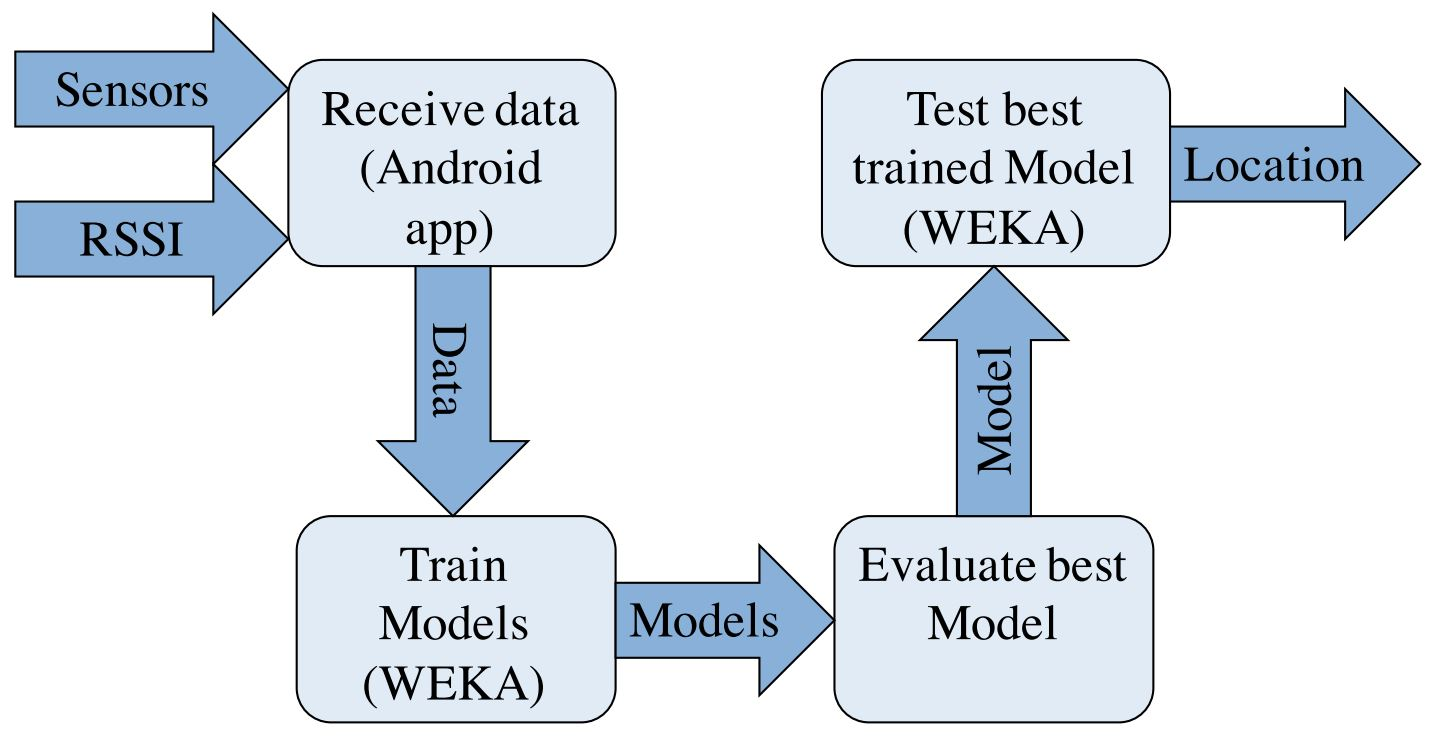
\includegraphics[width=100mm]{Figures/Architecture.jpg}
\decoRule
\caption[Architecture]{The architecture of the implemented android app.}
\label{fig:Architecture}
\end{figure}

%----------------------------------------------------------------------------------------
\section{Machine Learning Applications}

\subsection{Room Recognition}
In the room recognition phase we want the system to distinguish several rooms on the same floor. As mentioned above, the sensor accuracies are not high enough to enable the ability to distinguish data points collected at the border of two rooms. Our best practice was leaving one square metre of space at the doors without any data points collected.


\subsection{Landmark Recognition}
In the landmark recognition phase we want the system to distinguish several landmarks inside the room. As explained before, a landmark is defined as a small area within a room. Typically a landmark was of one square metre size and between each of the landmarks we left at least 2 metres space. This was our best practice and there may be better ways to do this. So in a small room (around 3x3 metres) we would have two landmarks, so one at each end. In a normal office-sized room (around 5x5 metres) we would have four landmarks, one in each corner. In a big room (around 7x7 metres) we would have five landmarks, one in each corner and one in the centre. In our experimental environment there were no bigger rooms available. (Figure \ref{fig:LandmarksChapter3})

\begin{figure}[H]
\centering
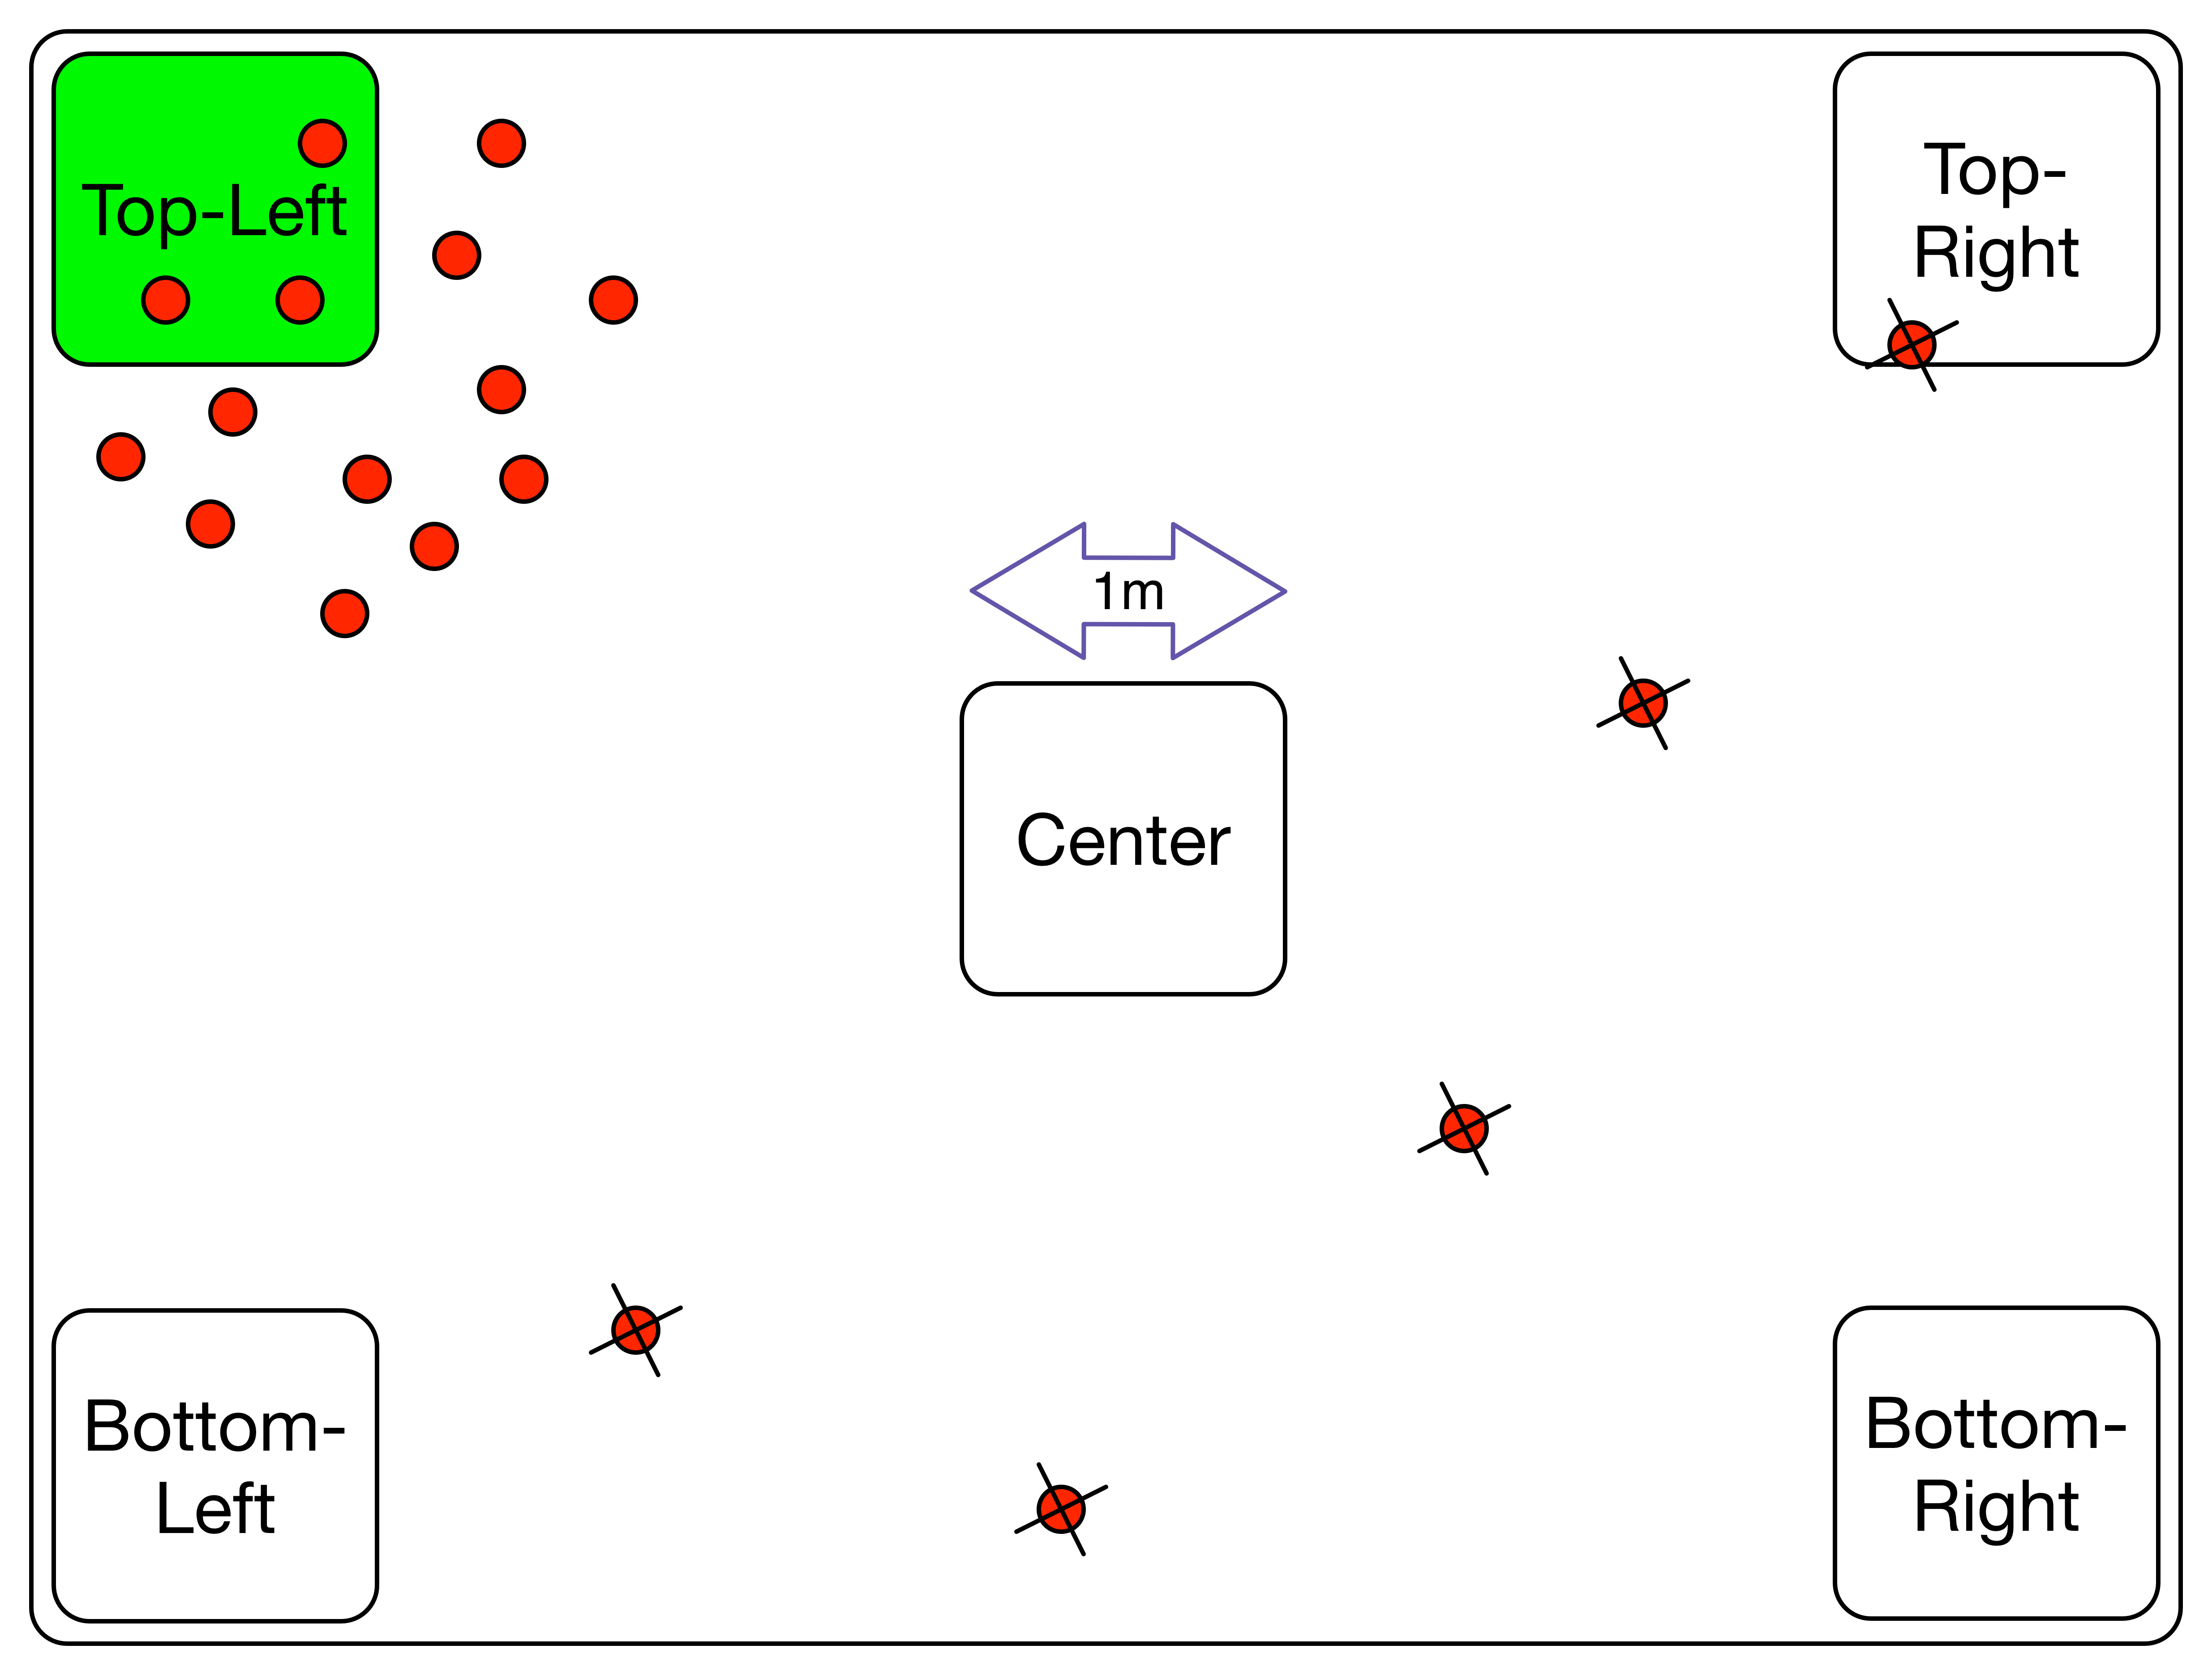
\includegraphics[width=100mm]{Figures/Landmarks.jpg}
\decoRule
\caption[Landmarks]{Five landmarks and the collection of red points predicted by the ITS.}
\label{fig:LandmarksChapter3}
\end{figure}


%----------------------------------------------------------------------------------------

\section{Data Collection Methodology}
\label{sec:DataCollection}

\begin{figure}[H]
\centering
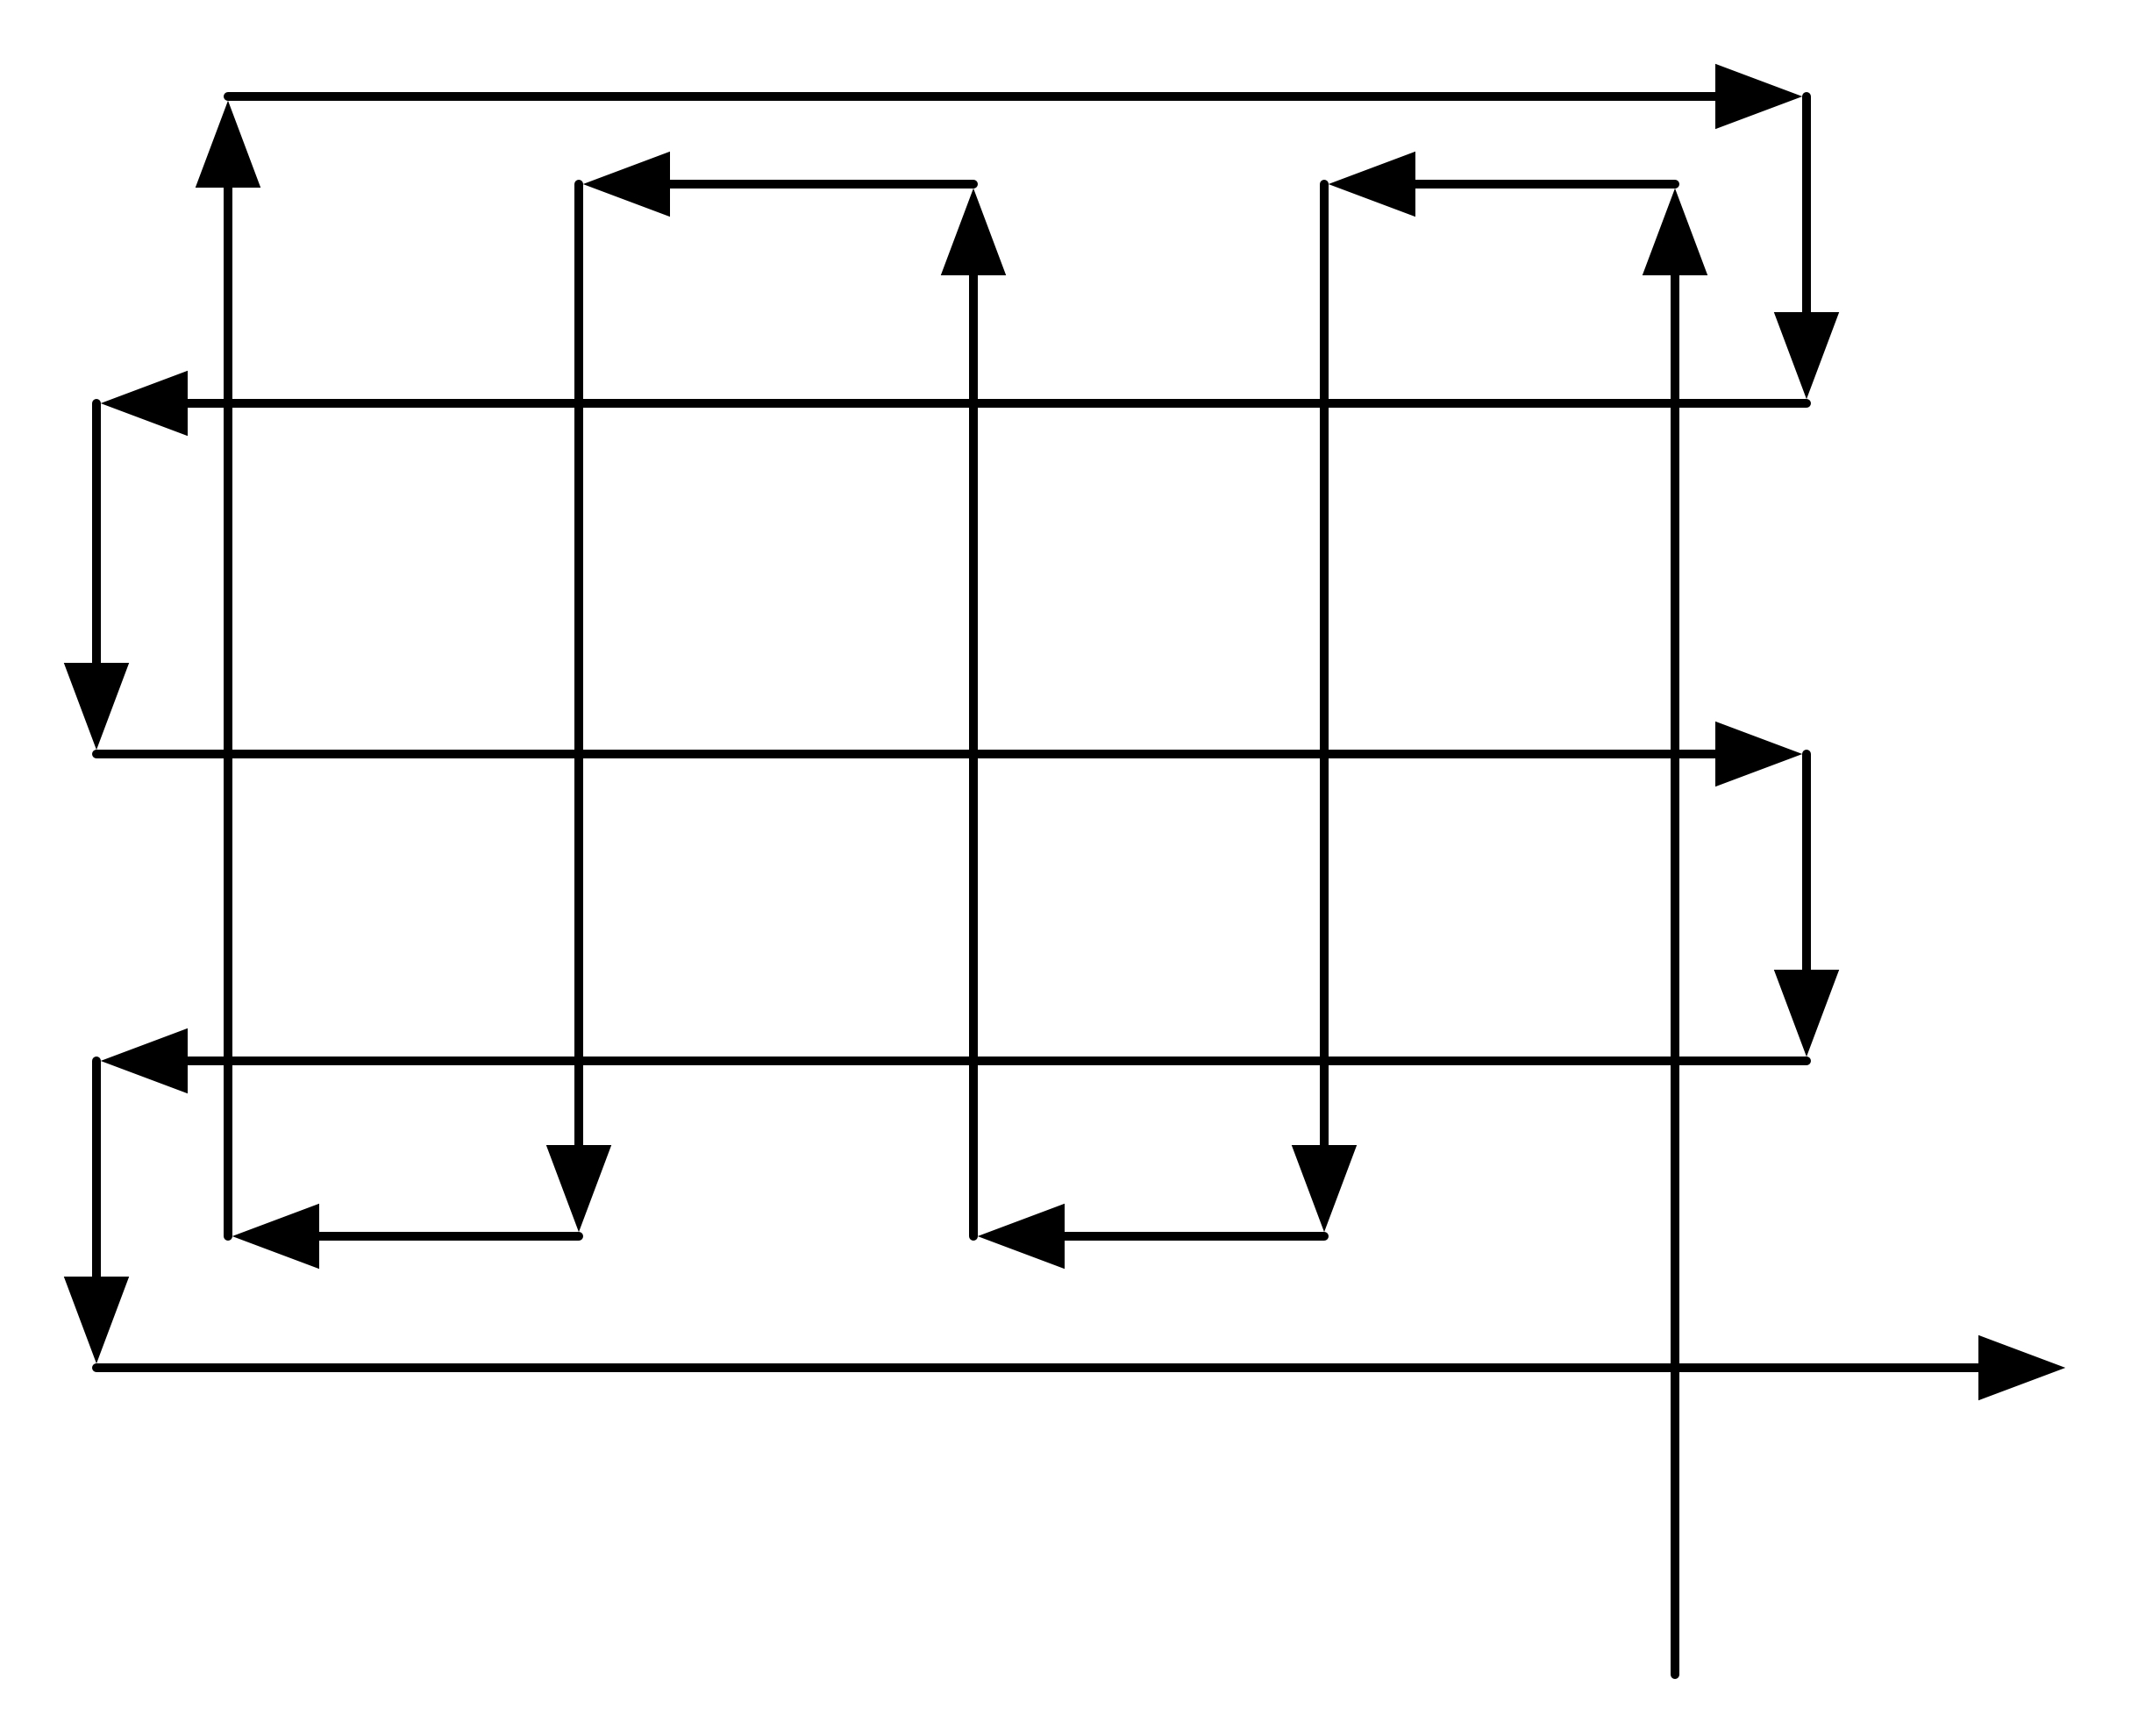
\includegraphics[width=100mm]{Figures/Grid.jpg}
\decoRule
\caption[Grid]{The grid pattern used to collect the data points.}
\label{fig:Grid}
\end{figure}
The data collection for both the training set and the test set have been done in a grid pattern, as shown in Figure \ref{fig:Grid}. So we started with the phone in one corner of the room or landmark respectively. Then, we continuously moved the phone back and forth in parallel vertical lines. Once we covered the entire area in vertical lines, we turned the device by 90 degrees and did the same in parallel horizontal lines until we arrived at the diagonally opposing corner. The distance between these lines was typically around 5cm. Using this grid pattern method, a very tightly woven net could be laid across the area. Therefore, the diversity of the collected data points could be maximized. Additionally, this way of collection data is very fast. For instance, it takes 20 minutes to finish the entire data collection in the third floor of institute building in Bern.

The training set and the testing set have been collected in two different gatherings within two hours on the same day. Because when they were collected in the same gathering and split up afterwards, Random Forest normally had over 99\% testing set accuracy in offline testing on the computer. But in live testing on the smart phone this accuracy was nowhere close (< 70\%). %The interested reader can see further information in the \href{https://github.com/JoelNiklaus/IndoLoc/blob/master/app/src/test/java/ch/joelniklaus/indoloc/experiments/OneDatasetTest.java}{One Dataset Test}  in my repository.

\begin{figure}[H]
\centering
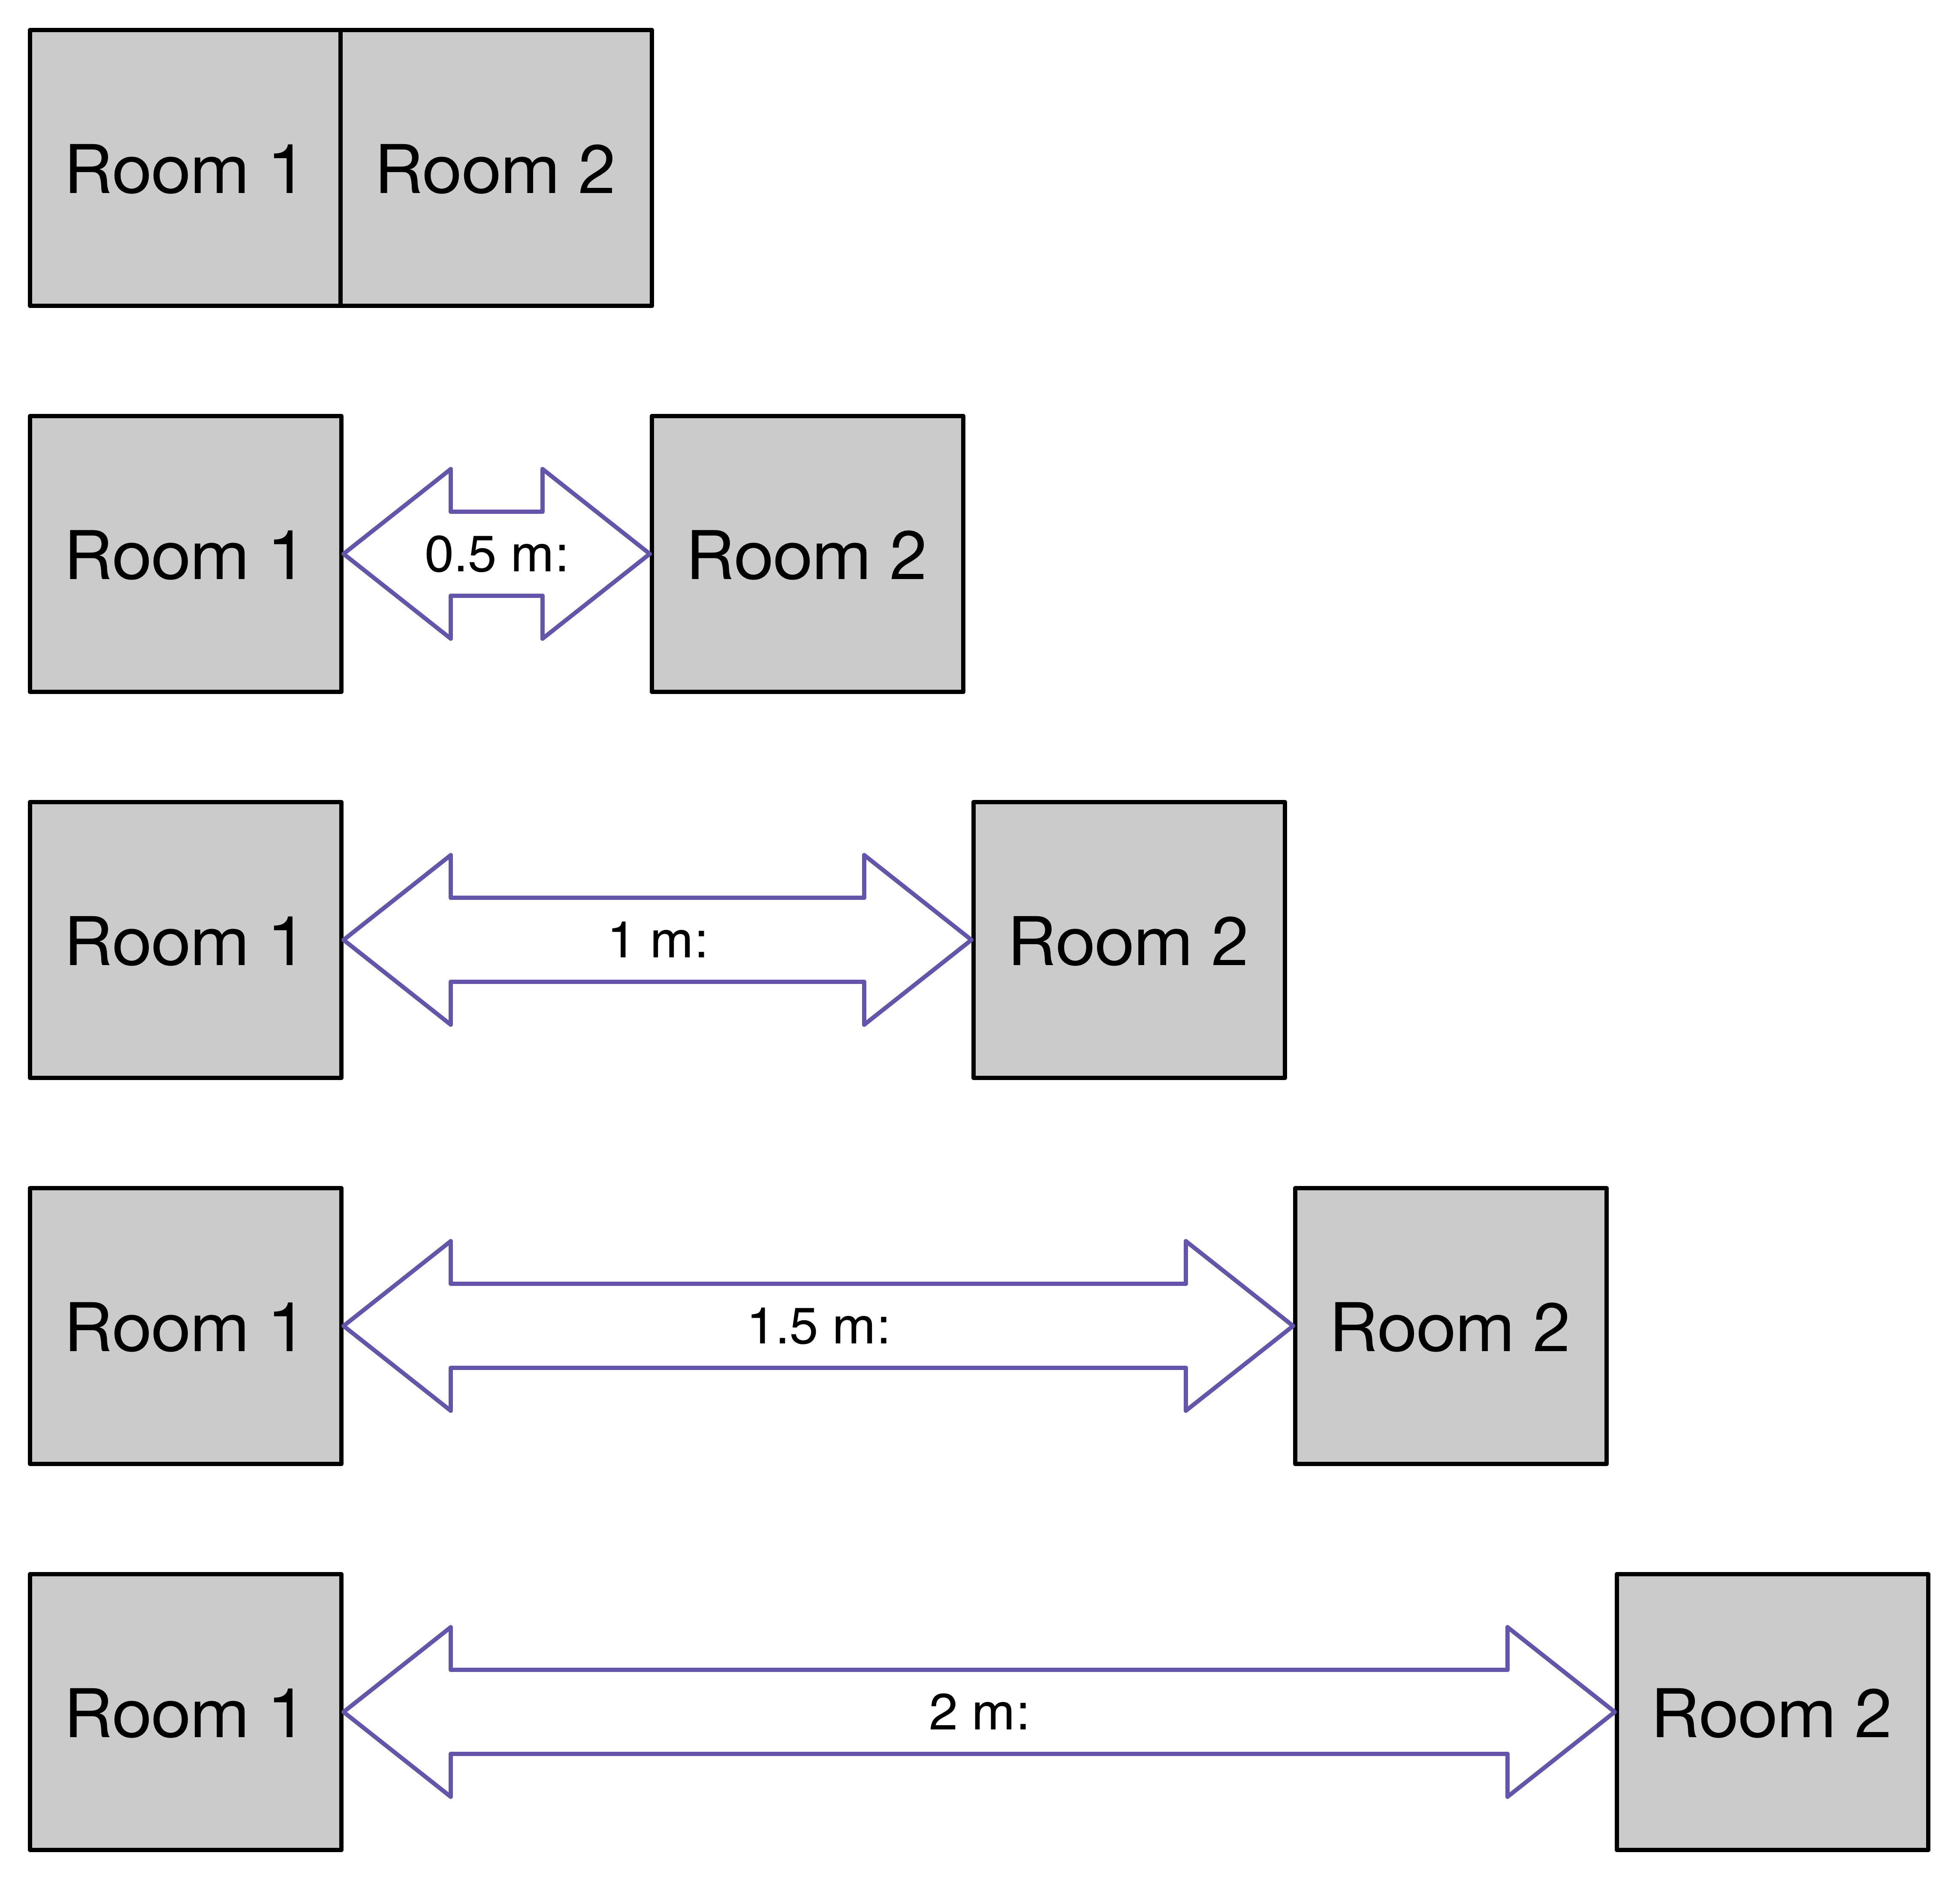
\includegraphics[width=100mm]{Figures/Distance.jpg}
\decoRule
\caption[Distance]{Distance between rooms.}
\label{fig:Distance}
\end{figure}

In supervised ML projects a class denotes the prediction output of the given ML algorithm. In our room prediction case the classes would be the different rooms and in analogy in our landmark prediction case the classes would be the different landmarks.

Generally, the physically closer together the classes are, the lower is the accuracy of the algorithms. This is due to small differences in the measured values (as shown in Figure \ref{fig:Distance}).

So on the one hand, when the distance between the classes is large, the measured values have greater differences between each other. This makes it easier to distinguish the classes and results in a higher prediction accuracy. However, this prediction is also less useful because there is a big uncategorized space in between the classes (as shown in the bottom row in Figure \ref{fig:Distance}).

On the other hand, if the distance between the classes is small, the measured values have smaller differences between each other. This of course exacerbates the problem of distinguishing the classes as the data points close to the border but in different classes have very similar values. But this prediction is much more helpful since more of the space can be categorized into a class (as shown in the top row in Figure \ref{fig:Distance}).
%But here we have to be careful, because if the prediction accuracy is not high enough we can assume that a high percentage of the mistakes the prediction makes are close to the border. 

So we have to find an optimal solution in between the two above extremes, which gives us a good accuracy but also does not come with too much uncategorized space.  Gathering from our experience we need an approximate distance of 1.5 metres between different classes to achieve an prediction accuracy of 85\%. 


In the method \texttt{registerListeners()} in the Sensor Helper class (on \url{https://github.com/JoelNiklaus/IndoLoc/blob/master/app/src/main/java/ch/joelniklaus/indoloc/helpers/SensorHelper.java}) we set the collection delay to \texttt{SENSOR\_DELAY\_NORMAL}. Looking at the Android Documentation (on \url{https://developer.android.com/guide/topics/sensors/sensors_overview.html}) we read that this delay is set to 200000 microseconds. Therefore, the sensor returns at least (!) 5 values per second.
% The WiFi collection rate is lower than the ones for the sensors.
So we collected around 5 data points per second walking at a constant rate.



%----------------------------------------------------------------------------------------
\section{Datasets}

A dataset consists of two separately collected subsets, the training and the test set. The training set usually is larger than the test set. Normally we use splits like 70\% training set and 30\% test set or 80\% and 20\%.

\subsection{Bern Dataset}
\label{sec:BernDataset}
The dataset considered for room recognition has been recorded on the third floor of the Computer Science building of the University of Bern at Neubrückstrasse 10, as shown in Figure \ref{fig:Bern}. It can be found on the github repository on \url{https://github.com/JoelNiklaus/IndoLoc/tree/master/app/src/main/assets/thesis/bern/room}.

\begin{figure}[H]
\centering
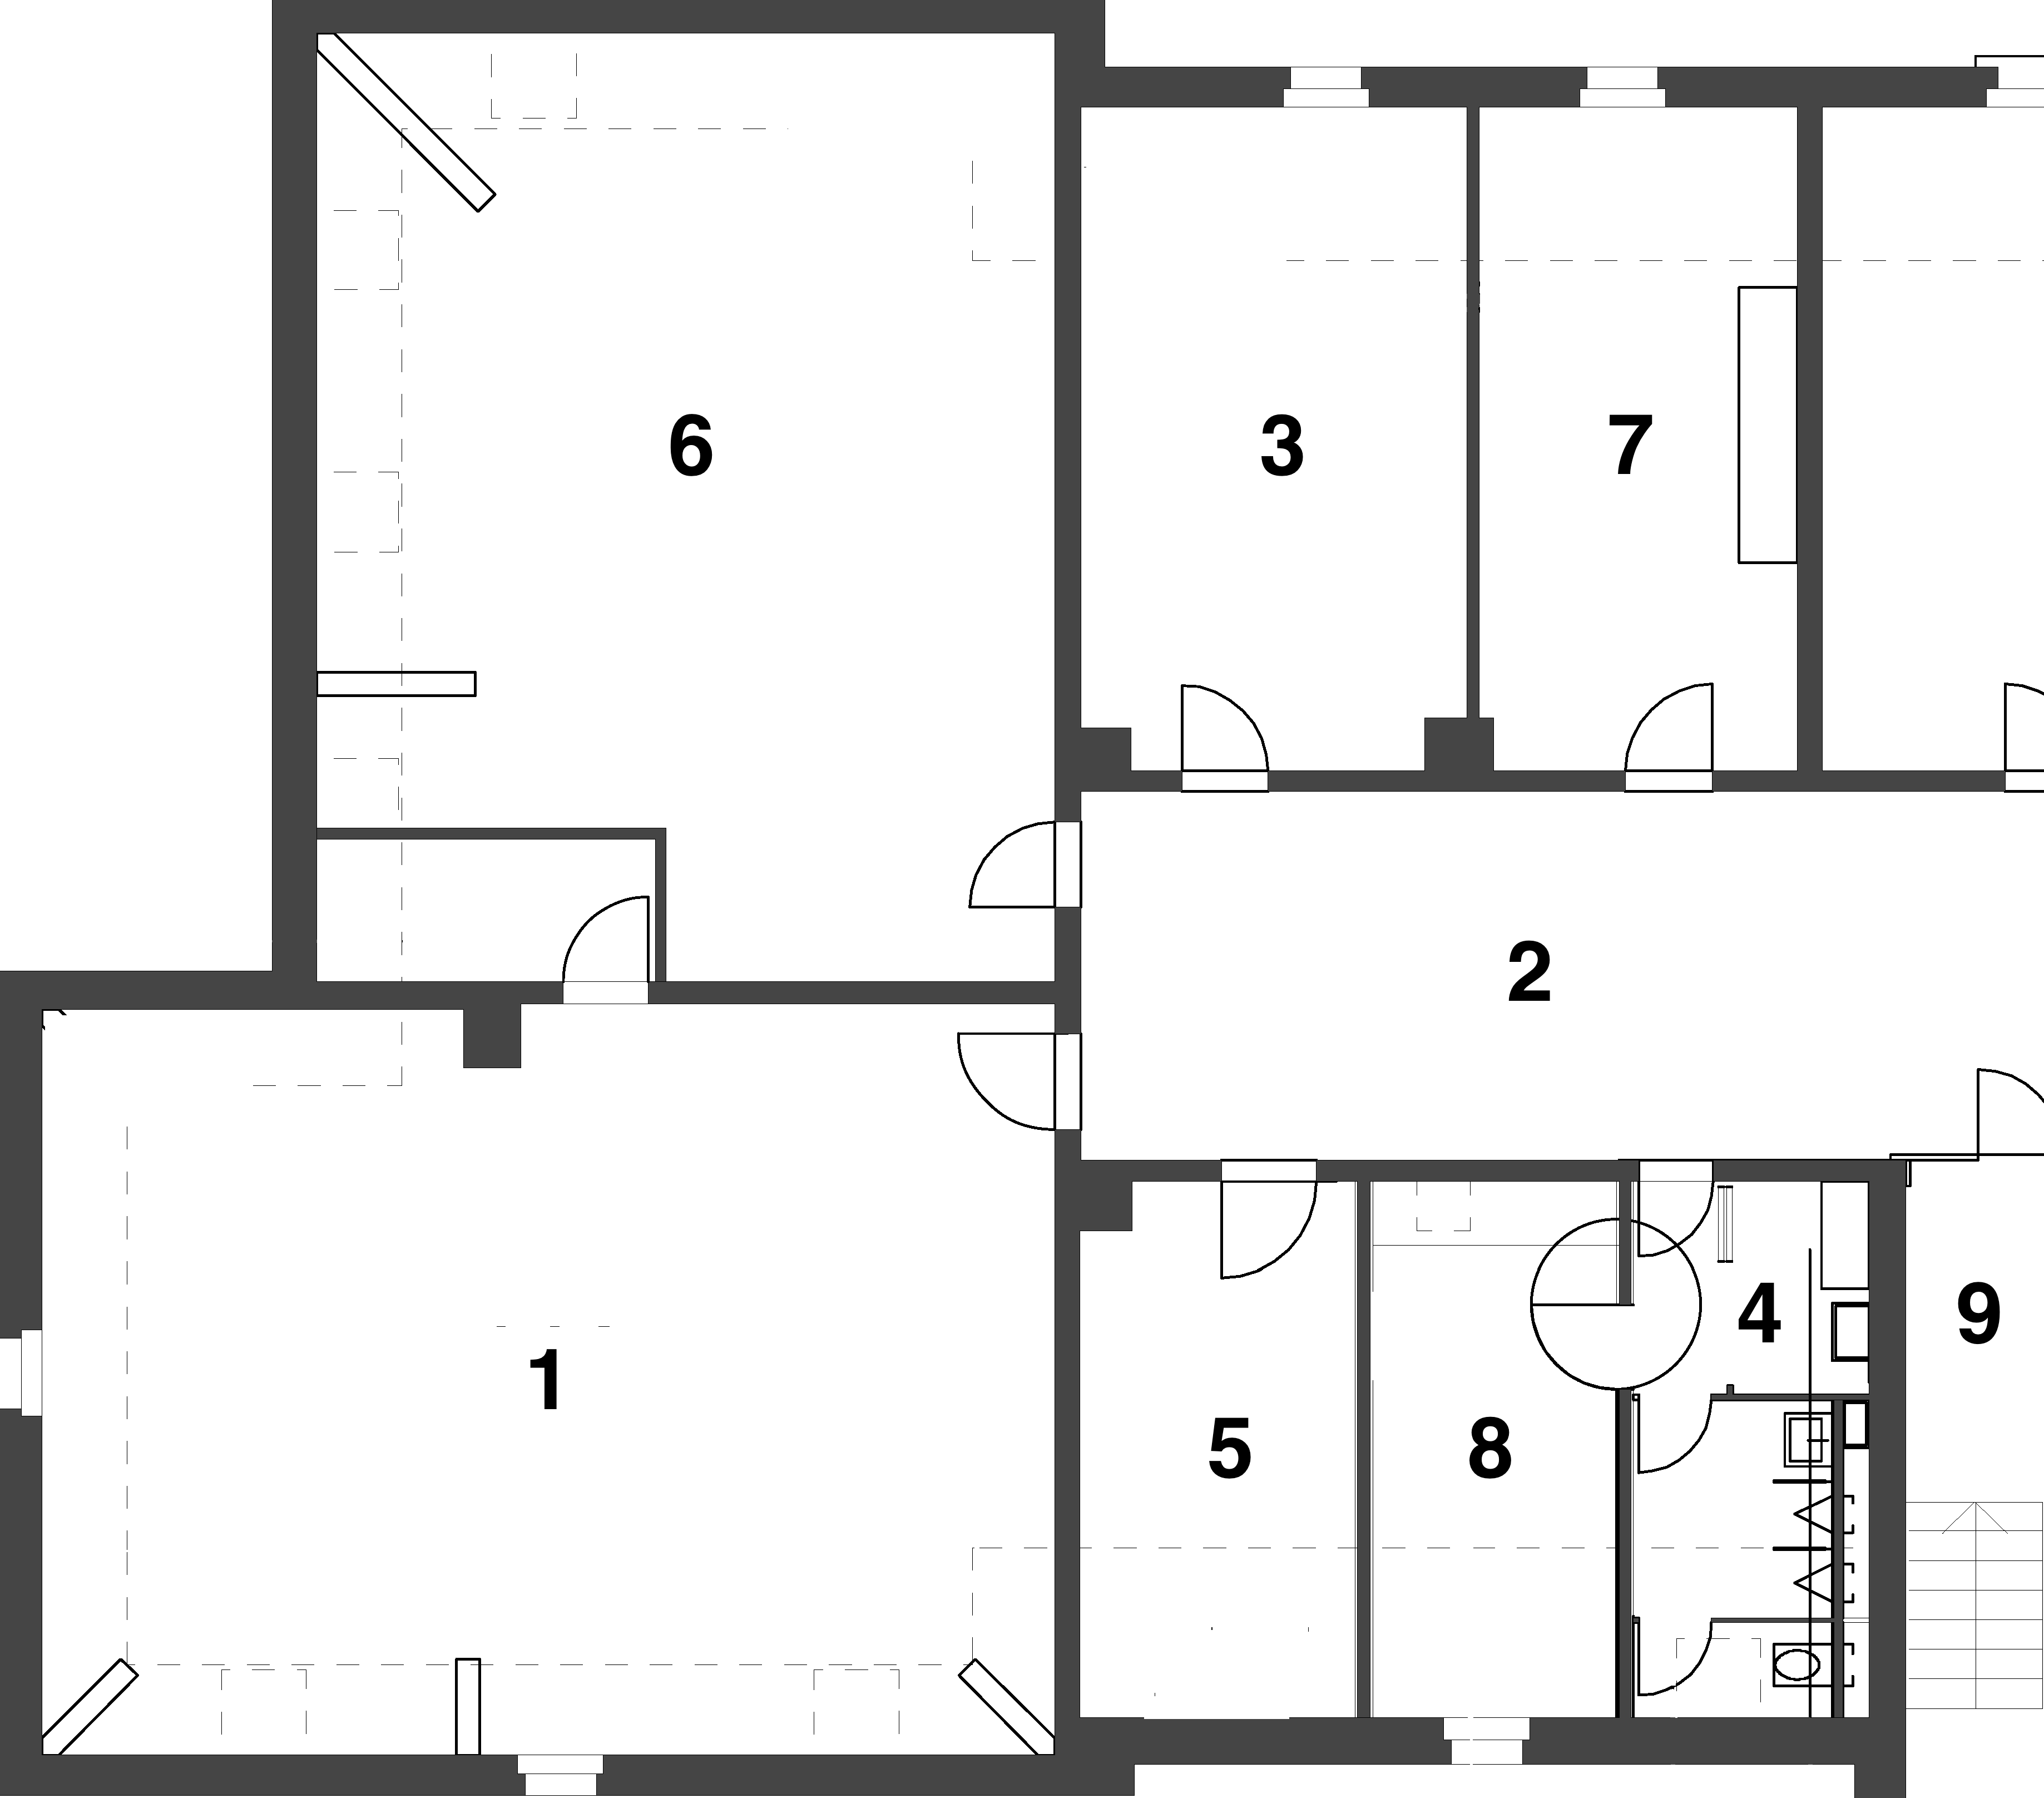
\includegraphics[width=100mm]{Figures/Bern.jpg}
\decoRule
\caption[Bern]{The testing environment in Bern.}
\label{fig:Bern}
\end{figure}

The training set contains 14569 data points in total. 3061 data points were collected in the biggest room (1) and 514 in the smallest room (4). As mentioned in Section \ref{sec:DataCollection} around 5 data points can be collected per second. Therefore, collecting the whole training set required around 50 minutes.

The test set contains 8624 data points with 2164 in room 1 and 291 in room 4. Collecting the whole test set required around 30 minutes.
In this dataset we collected all the features described above. So, in this section it is also described which of the features improve the accuracy and which of them could be left out.

This dataset is used to conduct experiments on room recognition level and on which features are beneficial for accuracy.

\subsection{Exeter Dataset}
\label{sec:ExeterDataset}
The dataset considered for landmark recognition has been recorded on the first floor of the living room in Block C in James Owen Court on Sidwell Street in Exeter, an apartment complex owned by the University of Exeter, as shown in Figure \ref{fig:Exeter}. It can be found on the github repository on \url{https://github.com/JoelNiklaus/IndoLoc/tree/master/app/src/main/assets/thesis/exeter/landmark}.

\begin{figure}[H]
\centering
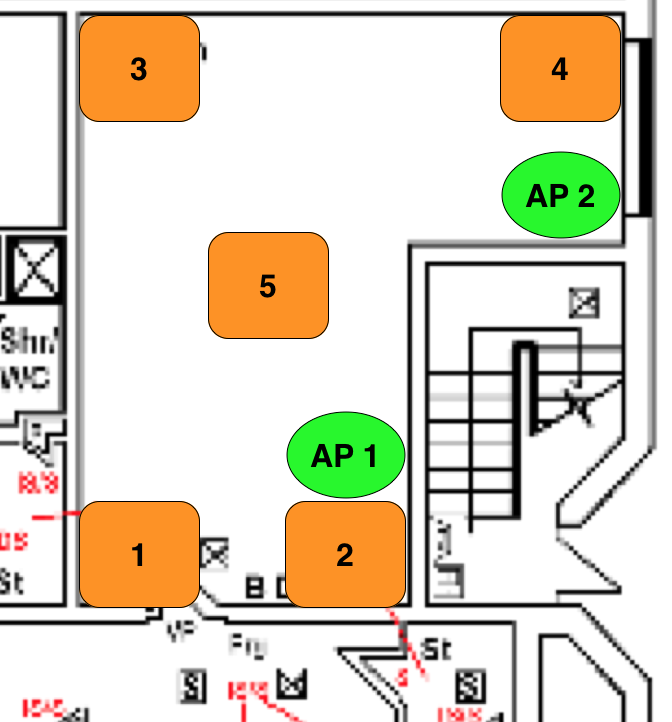
\includegraphics[width=100mm]{Figures/Exeter.jpg}
\decoRule
\caption[Exeter]{The testing environment in Exeter.}
\label{fig:Exeter}
\end{figure}



The training set contains 2522 data points in total. As each of the landmarks are of equal size we collected a little over 500 data points in each of them. Collecting the whole training set required approximately 10 minutes.

The test set consists of 1269 data points with a little over 250 data points in each landmark. Collecting the whole test set required approximately 5 minutes.

In this dataset we only collected the magnetic field values in the y and z directions, and the RSS values, because at the time of collection we presumed these to be important features. There are many different machine learning methods and they can each be parametrized in a variety of ways. Furthermore, each feature combination can be tested if it improves the result. So, in the following sections we am confining ourselves to the most expressive findings.

This dataset is used to conduct experiments on the landmark recognition level and to check if removing duplicates improves the result (\ref{sec:DuplicatesRemoval}).

%COMPARE WITH LANDMARK CDS!!

In every section there is a link available at the top which leads directly to the Java class doing the described experiment.

